\section{Laboratory model} \label{labModelSection}
In the GTAC laboratory there is a 96-loudspeaker array distributed as an irregular octagon (\autoref{WFSdistribution}), with the capability of performing WFS inside the area enclosed it. Hence, theoretically, if there are noise sources outside the area of the array, the field inside can be cancelled with the proper wave forms transmitted by the loudspeakers.

\begin{figure}
	\centering
	\reflectbox{\rotatebox[origin=c]{180}{
	\includegraphics[height=0.3\textheight]{./Img/WFSarraySchemeReport.pdf}
	}}
	\caption[WFS array distribution]{Schematic of the GTAC loudspeaker array distribution}
	\label{WFSdistribution}
\end{figure}

Previous \autoref{transEqMatrix} can be particularized to differentiate between loudspeakers that belong to the WFS array and the ones that produce noise:

\begin{equation}
	\vec{c_\mathit{micro}} = \myMatrix{A} \vec{c_\mathit{louds}} =
	\left. \begin{cases}
	\vec{c_\mathit{louds}} = 
	\begin{bmatrix}
		\vec{c_\mathit{WFS}} \\
		\vec{c_\mathit{NS}}
	\end{bmatrix} \\
	\myMatrix{A} =
	\begin{bmatrix}
		\myMatrix{A}_{WFS} & \myMatrix{A}_{NS}
	\end{bmatrix}
	\end{cases} \right\} =
	\myMatrix{A}_{\mathit{WFS}} \vec{c}_{\mathit{WFS}} + \myMatrix{A}_{\mathit{NS}} \vec{c}_{\mathit{NS}}
	\label{transEqMatrixRep1}
\end{equation}

%Matrix of acoustic paths $\myMatrix{A}$ can be calculated from theoretical parameters or from experimental results. The first case was already expressed in \refeq{acPathTheoric}:
%
%\begin{gather}
%a_{m,l} = \alpha_l D_{loud (l)}(\vec{r}_{loud (l)}, \vec{r}_{micro (m)}) G(\vec{r}_{loud (l)}, \vec{r}_{micro (m)}) D_{micro (m)}(\vec{r}_{loud (l)}, \vec{r}_{micro (m)}) \beta_m 
%\label{acPathTheoricRep1} \\
%\vec{r_\mathit{loud}} =
%\begin{bmatrix}
%	\vec{r_\mathit{WFS}} \\
%	\vec{r_\mathit{NS}}
%\end{bmatrix}
%\quad
%\vec{D_\mathit{loud}} =
%\begin{bmatrix}
%	\vec{D_\mathit{WFS}} \\
%	\vec{D_\mathit{NS}}
%\end{bmatrix} 
%\quad
%\vec{\alpha} =
%\begin{bmatrix}
%	\vec{\alpha_\mathit{WFS}} \\
%	\vec{\alpha_\mathit{NS}}
%\end{bmatrix}
%\label{WFSandNSconcatenation}
%\end{gather}
%
%The second case is:
%\begin{equation}
%a_{m, l} = \frac{c_{\mathit{micro} (m)}}{c_{\mathit{loud} (l)}}
%\end{equation}

Cancellation must be achieved through the manipulation of transmitted signals by the WFS array $\vec{c}_\mathit{WFS}$, since the noise signals $\vec{c}_{\mathit{NS}}$ are a given. A perfect cancellation would mean that the acoustic field inside the area is null. This is of course impossible in practice, not only because the chosen model is a simplification of the real scenario, but also because, even in ideal simplified conditions, an infinite number of infinitesimal sources would be required, as the theory states. However, we can aim to good enough cancellation levels. This means that the magnitude of the field would be reduced enough in most of the area inside the array. That would be reflected in the signals received by microphones placed inside the area ($\vec{c_\mathit{micro}}$). There are two main ways of doing it.

\subsection{Wave Field Synthesis in GTAC anechoic chamber} \label{WFSexplanation}
Cancellation can be achieved by means of using Wave Field Synthesis. This consists in generating the field that an hypothetical noise source (virtual noise source) equal to the real one but with opposite sign would produce. This way, both fields will cancel each other (the sum will be $0$).

WFS uses Kirchhoff integral as its mathematical principle. When Kirchhoff's integral is simplified and particularized to fit the scenario presented in the chamber (a finite number of discrete sources distributed as an octagon on a horizontal plane), some equations are deduced (\autoref{WFScalcEq} and \autoref{WFScalcEqDelay}). They use some of the theoretical parameters (position and coefficient of the noise source, position and orientation of the loudspeakers used for WFS) to calculate the transmitted coefficients ($\vec{c}_\mathit{WFS}$) of the solution. If loudspeakers can be modelled as monopoles and free-space conditions are guaranteed, we will achieve cancellation over the whole area. These calculations were provided by the professors and require much professional knowledge in the physic area, which is not an important section of the project.

The original noise signal is scaled by an attenuation coefficient and delayed a certain amount of time. The attenuation calculation requires the knowledge of the distance between the source and the loudspeaker $d$ and the angle $\alpha$ between the vector that goes from the source to the loudspeaker and the loudspeaker's broadside direction.
\begin{equation}
	\begin{aligned}
		\mu = 
		&\begin{cases}
		A\frac{\cos\alpha}{\sqrt{d}} & \alpha \leq 90^\circ \\
		0 & \alpha > 90^\circ
		\end{cases}
		\\
		A &= \sqrt{\frac{r_0}{r_0 + d}}\\
		r_0 &= \frac{1.44}{2} + 1.44 \cos\left( \frac{\pi}{4} \right)
	\end{aligned}
	\label{WFScalcEq}
\end{equation}
Beware there is a condition that must be fulfilled for a loudspeaker to be active: if the angle $\alpha$ is smaller than $90^\circ$ (\autoref{figAngleCondition}), then the loudspeaker is active. In other case, is not enabled.

%	\input{./Img/pruebaSVGLatex.pdf_tex}
\begin{figure}
	\centering
	\def\svgwidth{0.4\columnwidth}
	\graphicspath{{Img/}}
	\input{Img/WFSParameters.pdf_tex}
	\caption[WFS calculation parameters]{WFS calculation parameters}
	\label{figAngleCondition}
\end{figure}

The delay time is actually the time it takes for the sound transmitted by the noise source to reach the loudspeaker. It is related to the distance $d$ and the propagation velocity of acoustic waves in air $c = 343 (m/s)$.
\begin{equation}
	\tau = \frac{d}{c} \label{WFScalcEqDelay}
\end{equation}

For a given distribution of loudspeakers, the coefficients of the signals that must be transmitted ($\cwfs$) depend only on the assumed characteristics of the virtual noise sources, this is, their position ($\vec{r}_{NS, n}^v,\, n = 1, \ldots, \numNS$) and the coefficients of the signals they transmit ($\cns^v$). If we call $\mu_{m,n}$ and $\tau_{m,n}$ to the attenuation and delay that the $m$-th loudspeaker applies to the $n$-th noise signal, and take into consideration only one frequency $f$:

\begin{equation}
\cwfs = 
 \left\{ \wfsNormCoef[mat] = \begin{bmatrix}
\wfsNormCoef[scalar]_{1,1} & \ldots & \wfsNormCoef[scalar]_{1,\numNS} \\
\vdots & \ddots & \vdots \\
\wfsNormCoef[scalar]_{\numWFS,1} & \ldots & \wfsNormCoef[scalar]_{\numWFS,\numNS}
\end{bmatrix},\quad \wfsNormCoef_{n,m} = -\mu_{n,m} e^{-j 2 \pi f \tau_{m,n}} 
\right\}
= \wfsNormCoef[mat] \cns^v
\end{equation}

Nonetheless, the real scenario is not ideal. The coefficients calculated with the previous method don't always produce a good enough cancellation when the acoustic paths are not the ideal ones. Then, some form of numerical optimisation can be useful.

\subsection{Optimization} \label{optimization}
In order to perform the optimisation, we've followed the usual concept of defining an objective function that returns a number depending on some of inputs, and then finding the inputs that minimize the function.

\begin{equation}
[x_{\mathit{opt} (1)}, x_{\mathit{opt} (2)}, ..., x_{\mathit{opt} (N)}] = \argmin_{x_1, x_2, ..., x_N} f(x_1, x_2, ..., x_N)
\label{optimisationGeneral}
\end{equation}

A simple and useful objective function is the norm of the vector of received signal coefficients $\norm{\vec{c_\mathit{micro}}}$. The optimization is then:
\begin{gather}
\vec{c_{\mathit{WFS}, \mathit{opt}}} =
\argmin_{\vec{c_\mathit{WFS}}}
\norm{\vec{c_\mathit{micro}}} =
\argmin_{\vec{c_\mathit{WFS}}}
\norm{\myMatrix{A}
\begin{bmatrix}
\vec{c_\mathit{WFS}}\\
\vec{c_\mathit{NS}}\\
\end{bmatrix}
} \\
\left | \vec{c_{\mathit{WFS}}} \right | <= 1
\label{OptConstraint}
\end{gather}

The solution could easily be calculated by solving the linear system. In case there aren't more microphones than loudspeakers, perfect cancellation at those points will be achieved. In case there are more microphones than loudspeakers, we just use the Moore-–Penrose inverse to solve the overdetermined linear system. However, depending on the situation, we might want to set a constraint that limits the amplitude of coefficients to $1$ (\autoref{OptConstraint}), since a digital signal that exceed that value would produce audio clipping. This forces us to use some form of numeric non-linear optimisation, as the interior point algorithm.

It should be noted that, while the equations derivated from Kirchhoff's integral are intended to produce cancellation over the whole area, the optimisation is applied only to a finite number of discrete points. So, the spatial distribution of those points will affect the final result.

This solution doesn't take in account any physical knowledge of the scenario, nor the WFS techniques. It's just a solution to a system of linear equations. A half way approach to this, is to minimize the same parameter $\norm{\vec{c_\mathit{micro}}}$, but not changing the transmitted coefficients $\vec{c_{\mathit{WFS}}}$ directly. Instead, we apply the constraint that they must be generated by the WFS calculation that we talked about previously (\autoref{WFSexplanation}). In other words, we find the virtual noise source parameters that would produce the greatest cancellation for a finite set of points. This can be useful to compare how much the real scenario can be approximated by an ideal one. For simplification, let's consider just one noise source:

\begin{equation}
[\cnsScalar^v, \vec{r_{\mathit{NS}}^v}] =
\argmin_{\cnsScalar^v, \vec{r_{\mathit{NS}}^v}}
\norm{\myMatrix{A}
	\begin{bmatrix}
	\vec{c_\mathit{WFS}}(\cnsScalar^v, \vec{r_{\mathit{NS}}^v})\\
	\cnsScalar\\
	\end{bmatrix}
} =
\argmin_{\cnsScalar^v, \vec{r_{\mathit{NS}}^v}}
\norm{\myMatrix{A}
	\begin{bmatrix}
	\wfsNormCoef[mat](\vec{r_{\mathit{NS}}^v})\cnsScalar^v\\
	\cnsScalar\\
	\end{bmatrix}
}
\end{equation}

It could be that the cancellation at some points was more of a priority than at some others. For example, achieving cancellation in the centre of the area is more important than the region near the border, or it could be that we wanted to compensate for the difference in the response of microphones. In those cases we can just multiply each row of $\myMatrix{A}$ by a correction coefficient.

Evaluating the result consists of calculating the power of the received signals in the optimized case.
\begin{gather}
	\vec{p_\mathit{micro,opt}} = \frac{\abs{\vec{c_{\mathit{micro,opt}}}}^{\circ 2}}{2}
	\\
	\vec{c_\mathit{\mathit{micro,opt}}} = \myMatrix{A}
	\begin{bmatrix}
	\vec{c_\mathit{WFS,opt}} \\
	\vec{c_{\mathit{NS}}}
	\end{bmatrix}
\end{gather}

However, that result makes not much sense if we don't compare it to the power of noise we would have if there was no cancellation. So, interesting results are the signal power and the cancellation $\vec{C}$ defined as:

\begin{gather}
\vec{C} = \vec{p_\mathit{micro,opt}} \oslash \vec{p_\mathit{micro,NS}} \\
\vec{p_\mathit{micro,NS}} = \frac{\abs{\vec{c_{\mathit{micro,NS}}}}^{\circ 2}}{2}\\
\vec{c_{\mathit{micro,NS}}} = \myMatrix{A} 
\begin{bmatrix}
	\vec{0} \\
	\vec{c_{\mathit{NS}}}
\end{bmatrix}
\end{gather}

Another interesting result comes from comparing the sum of the power of all received signals with and without cancellation, like some sort of global cancellation $C_\mathit{global}$:
\begin{equation}
C_\mathit{global} = \frac{\norm{\vec{p_\mathit{micro,opt}}}_1}{\norm{\vec{p_\mathit{micro,NS}}}_1}
\end{equation}

\subsection{Visualizing of results}
In order to visualize the results, two ways have been used. The first one uses two histograms with logarithmic scale that shows how the power and cancellation of the different received signals are distributed. It also returns parameters as the mean, maximum, minimum, standard deviation. In addition, it shows the global cancellation.

The second way is by using a 2D map of the lab scenario. The points were the microphones are located appear as circles filled with a colour that depends on the power or cancellation levels. Loudspeakers also appear with some colour depending on the power of the transmitted signals.

\section{Experiment 1: GTAC acoustic paths}
The first experiment is a completely theoretical one, although it uses results from previous measures. The acoustic responses in the GTAC laboratory for different points was measured with high precision previously, and the results are published in the website. In total, the measures were done in 360 points distributed in a rectangular grid of size $24$x$15$ and separation of $20 \si{cm}$ between adjacent nodes (\autoref{GTAC360micro}).

\begin{figure}
	\centering
	\reflectbox{\rotatebox[origin=c]{180}{
			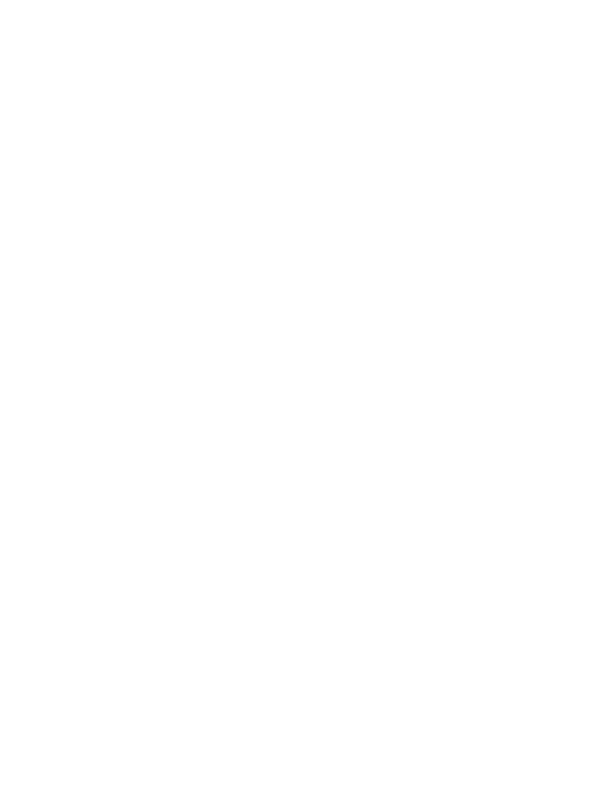
\includegraphics[height=0.3\textheight]{./Img/WFSGTAC360microphones.pdf}
	}}	
	\caption[Schematic of measures in GTAC anechoic chamber]{Schematic of measures in GTAC anechoic chamber}
	\label{GTAC360micro}
\end{figure}

%We could apply the optimization already described in \autoref{optimization}, but there is a problem. GTAC responses are measured for loudspeakers in the WFS array, but of course, not for loudspeakers outside the array in arbitrary positions. Hence, we can only guess the acoustic paths by applying the theoretical model (\autoref{acPathTheoric}), in which case we assume that the noise source is isotropic. Then, we apply the optimization process and see how far we can go in the cancellation. Only the first type of optimization is interesting since the position of the noise loudspeaker is known.

GTAC responses are measured for loudspeakers in the WFS array, but of course, not for loudspeakers outside the array in arbitrary positions. Hence, we can only guess the acoustic paths by applying the theoretical model (\autoref{acPathTheoric}), in which case we assume that the noise source is isotropic.

Results are shown in \reffig{}. Different positions have been used. As we can see, cancellations of X dB are easy to achieve.

\section{Experiment 2: theoretical simulation}
The

\section{Experiment 3: lab recording}






